\documentclass{article}
\usepackage[utf8]{inputenc}

\usepackage{amsmath}
\usepackage{amssymb}
\usepackage[T1]{fontenc}
\usepackage{graphicx}
\usepackage{physics}
\usepackage{siunitx}
\usepackage{textcomp}
\usepackage{bm} %Negrita en ecuaciones.
\usepackage{enumerate} %para usar romanos en enumerate.
\usepackage{gensymb} %Para usar \degree.
\usepackage{geometry} %Para editar los margenes.
\geometry{right=15mm,left=15mm,top=25mm,bottom=25mm}
\usepackage{fancyhdr} %Encabezado y Pie de Pagina.
\usepackage{lastpage} %LastPage.
\pagestyle{fancy}
\setlength{\headheight}{15pt} 
\lhead{Consurso - Física Arq/Física I}
\rhead{Juan Francisco Viso}
\cfoot{}
\rfoot{\thepage\ / \pageref{LastPage}}
\renewcommand{\headrulewidth}{1pt}
\renewcommand{\footrulewidth}{1pt}
\usepackage{wrapfig} %para colocar imagenes al lado de los párrafos.
\usepackage{multicol} %para poner columnas
\usepackage{tikz} %Para dibujar!


\author{Juan Francisco Viso	}
\title{Concurso - Física Arq/Física I}
\date{April 2018}

\begin{document}

\begin{center}
{\huge \textbf{Concurso - Física Arq/Física I} \par}
{\LARGE \textbf{Dinámica de Fluidos, Ecuación de Continuidad\\ y Ecuación de Bernoullie} \par}
\rule{\linewidth}{.3pt}
\end{center}

\begin{enumerate}
\item El movimiento de un fluido se puede dividir en dos tipos: \textit{laminar} o \textit{turbulento}.
\item Un fluido es \textit{laminar} si todas las partículas que pasan por un punto del fluido se mueven por el mismo camino suave que las particulas anteriores.
\item Un fluido es ideal si:
\begin{enumerate}[I.]
\item Es incompresible, es decir su densidad es constante.
\item Su viscosidad es nula, por lo tanto no pierden energía por fricción.
\item El movimiento del fluido es estacionario, es decir, su velocidad, presión y densidad en cada punto del fluido es constante.
\item El movimiento no es turbulento, no hay corrientes de Eddy.
\end{enumerate}
\end{enumerate}

\large{\textbf{Ecuación de Continuidad}}
\begin{gather*}
m_1\ =\ m_2 \\
\rho_1 V_1\ =\ \rho_2 V_2\ \\
\rho_1 A_1\ \Delta x_1 =\ \rho_2 V_2\ \Delta x_2 \\
\rho_1 A_1\ v_1 \Delta t =\ \rho_2 V_2\ v_2 \Delta t \\
A_1 v_1\ =\ A_2 v_2
\end{gather*}

Esta ecuación nos dice que la sección de un fluido disminuye a medida que aumenta la velocidad del mismo. Al factor $Av$ que tiene unidades de $\frac{m^3}{t}$ se lo denomina \textbf{flujo}.

\vspace{0.5cm}
\large{\textbf{Ecuación de Bernoullie}}

La ecuación de Bernoullie puede deducirse a partir del \textit{Teorema de las fuerzas vivas}, calculando el trabajo realizado por la diferencia de presión entre los extremos del volumen de control y teniendo en cuenta el trabajo realizado por las fuerzas conservativas (como la gravedad) cuyo trabajo es igual a la variación de la energía potencial. De esta manera, obtenemos:
\begin{equation*}
\Delta T\ =\ W_{Conservativo}\ +\ P_1 A_1 L_1\ -\ P_2 A_2 L_2
\end{equation*}
Luego, como $AL$ es igual al volumen y ambos volumens son iguales devido a que el fluido es incompresible, obtenemos que el trabajo realizado por la fuerza asociada a la presión es igual a:
\begin{equation*}
(P_1 - P_2)V
\end{equation*}
Finalmente dividiendo a cada termino por la masa total del volumen de control y recordando que la densidad es $\rho=m/V$ y que la misma es constante, obtenemos la ecuación de Bernoullie:
\begin{equation*}
P\ +\ \frac{1}{2}\rho v^2\ + \rho g h\ =\ cte
\end{equation*}

\pagebreak
\noindent{\large{\textbf{Problema 1}}}

\noindent{En un deposito herméticamente cerrado de gran sección, la altura del agua salada que contiene alcanza una altura de 3.2 m. El deposito contiene aire comprimido a una presión manométrica de 7000 Pa. El tubo horizontal de salida tiene una sección de 16 y 8 cm2 en las partes ancha y delgada respectivamente.}

\vspace{0.5cm}
\hspace{-0.7cm}
\begin{minipage}{0.65\textwidth}
\begin{enumerate}[a)]
\item ¿Cuál es la velocidad del fluido en el tubo angosto?
\item ¿Cuál es el caudal de salida por el tubo angosto?
\item ¿Qué altura \textbf{h} alcanzara el agua en el tubo vertical (manométrico)?
\end{enumerate}
\textit{Nota: Densidad relativa del agua salada: 1.035.}
\end{minipage}
\begin{minipage}{0.4\textwidth}
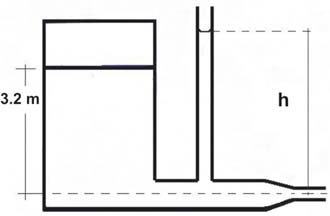
\includegraphics[width=0.9\textwidth]{imagen2.png}
\end{minipage}
\bigskip

\noindent{\large{\textbf{Problema 2}}}

\noindent{El tubo de Venturi de la gura tiene sección transversal de 30 $cm^2$ en las parte ancha, y de 10 $cm^2$ en el estrechamiento. Cada 5 segundos salen del tubo 25 litros de agua.}

\vspace{0.5cm}
\hspace{-0.7cm}
\begin{minipage}{0.65\textwidth}
\begin{enumerate}[a)]
\item Calcular las velocidades del agua en las partes ancha y angosta.
\item Hallar la diferencia de presión entre estas secciones.
\item Calcular la diferencia de altura entre las columnas de mercurio del tubo en U.
\end{enumerate}
\textit{Nota: $Hg = 13600\ kg/m^3$ y $H_2O = 1000\ kg/m^3$}
\end{minipage}
\begin{minipage}{0.35\textwidth}
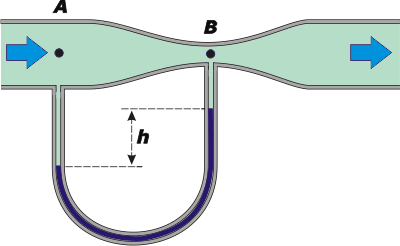
\includegraphics[width=1.0\textwidth]{imagen1.png}
\end{minipage}
\bigskip

\noindent{\large{\textbf{Problema 3}}}

\noindent{Una fuente de jardín arroja un chorro de agua vertical, con un caudal Q = 4 litros/s, alcanzando una altura de 2.4 m. No tenga en cuenta los efectos de turbulencia ni la desintegración del chorro.}
\begin{enumerate}[a)]
\item Calcular la velocidad inicial del chorro.
\item Calcular el radio del agujero por el que sale el agua.
\item Calcular la velocidad del chorro a una altura de 0.8 m.
\item Calcular el radio de la sección transversal del chorro de agua.
\end{enumerate}

\end{document}



